\section{Construção dos modelos} 

% ----------------------------

\begin{frame}{\textit{Modelo PE}: Características do fluido}
	\begin{itemize}
		\item \textbf{Homogêneo.} A densidade do fluido é uniforme em todo volume;
		\item \textbf{Incompressível.} O volume não muda quando submetido à pressão.
	\end{itemize}
\end{frame}

% ----------------------------

\begin{frame}{\textit{Modelo PE}: O modelo de água rasa}
		
	Fazendo as devidas alterações notacionais em \cite{salmon1998}, temos:
	\begin{align}
		\frac{\partial V}{\partial t} + (V \cdot \nabla)V + f \mathbf{k} \times V & = -g \nabla z \label{eq:agua-rasa-1} \\
		\frac{\partial z}{\partial t} + \nabla \cdot (z V)                        & = 0 \label{eq:agua-rasa-2}           
	\end{align}
		
	\begin{small}
		Onde:
		\begin{multicols}{2}
			\begin{itemize}
				\item $t$: tempo;
				\item $\mathbf{r}$: vetor de posição inicial;
				\item $V(t,r)$: Velocidade horizontal;
				\item $z(t,r)$: altura da superfície;
				\item $f$: parâmetro de Coriolis;
				\item $g$: aceleração da gravidade;
				\item $\mathbf{k}$: vetor da vertical.
			\end{itemize}
		\end{multicols}
	\end{small}
\end{frame}

% ----------------------------

\begin{frame}{\textit{Modelo PE}: O modelo de água rasa modificado}
	\begin{small}
		No artigo, são apresentadas as seguintes equações:
		\begin{align}
			\frac{\partial V}{\partial t} & = - ( V \cdot \nabla)V - f \mathbf{k} \times V - g \nabla z + \nu \nabla^2\mathbf{V} \label{eq:agua-rasa-modificada-1}     \\
			\frac{\partial z}{\partial t} & = - (V \cdot \nabla)(z - h) - (H + z - H)\nabla \cdot \mathbf{V} + \kappa \nabla^2 z + F \label{eq:agua-rasa-modificada-2} 
		\end{align}
	\end{small}
	\begin{scriptsize}
		Onde:
		\begin{multicols}{2}
			\begin{itemize}
				\item $t$: tempo
				\item $\mathbf{r}$: vetor de posição inicial;
				\item $H$: profundidade média do fluido;
				\item $h(r)$: variação da superfície topológica;
				\item $V(t,r)$: Velocidade horizontal;
				\item $z(t,r)$: altura da superfície;
				\item $f$: parâmetro de Coriolis;
				\item $g$: aceleração da gravidade;
				\item $F$: forças externas;
				\item $\kappa$: coeficiente de difusão viscosa;
				\item $\nu$: coeficiente de difusão térmica;
				\item $\mathbf{k}$: vetor da vertical.
			\end{itemize}
		\end{multicols}
	\end{scriptsize}
\end{frame}


% ----------------------------

\begin{frame}{\textit{Modelo PE}: Modelo de água rasa}


\begin{center}
    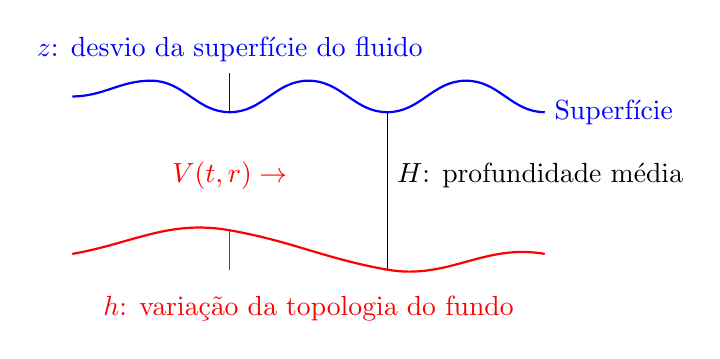
\begin{tikzpicture}
    \draw[blue, thick] (0,4) to[out=0,in=180] (1,4.2) 
                            to[out=0,in=180] (2,3.8)
                            to[out=0,in=180] (3,4.2)
                            to[out=0,in=180] (4,3.8)
                            to[out=0,in=180] (5,4.2)
                            to[out=0,in=180] (6,3.8);
    \node[blue, right] at (6,3.8) {Superfície};
    
    % Anotação do desvio z - agora apontando para cima a partir do vale
    \draw[blue] (2,3.8) -- (2,4.3);  % Linha vertical para cima a partir do vale
    \node[blue] at (2,4.6) {$z$: desvio da superfície do fluido};
    
    % Velocidade V(t,r)
    \node[red] at (2,3) {$V(t,r) \rightarrow$};
    
    % Profundidade média H
    \draw[black] (4,3.8) -- (4,1.8);
    \node[right] at (4,3) {$H$: profundidade média};
    
    % Topologia do fundo (curva inferior)
    \draw[red, thick] (0,2) to[out=10,in=170] (2,2.3) to[out=350,in=170] (4,1.8) to[out=350,in=170] (6,2);
    
    % Variação h
    \draw[red] (2,2.3) -- (2,1.8);
    \node[red] at (3,1.3) {$h$: variação da topologia do fundo};

\end{tikzpicture}
\end{center}

\end{frame}

% ----------------------------

\begin{frame}{\textit{Modelo PE}: Sobre os processos de difusão}
	Nas equações \eqref{eq:agua-rasa-modificada-1} e \eqref{eq:agua-rasa-modificada-2}, temos dois processos de difusão:
	\begin{enumerate}
		\item \textbf{Difusão viscosa:} transferência do momento entre partes do fluido devido à viscosidade \textit{(exemplo: mel)};
		\item \textbf{Difusão térmica:} Transferência de calor por condução entre regiões com diferentes temperaturas.
	\end{enumerate}
		
	\begin{small}
	    \textit{Observação: Ambos os processos tendem a uniformizar suas respectivas propriedades.}
	\end{small}
\end{frame}

% ----------------------------
\begin{frame}{\textit{Modelo PE}: Algumas observações das equações \eqref{eq:agua-rasa-modificada-1} e \eqref{eq:agua-rasa-modificada-2}}
	\begin{enumerate}
		\item A média horizontal de $h$ e $z$ é zero;
		\item $V(t,r)$ e $z(t,r)$ são amortecidas pelo processo de difusão de pequenas escala, este fato auxilia na simulação de fenômenos atmosféricos;
		\item O ``efeito $\beta$'', efeito que indica como o movimento do fluido é afetado pelas alterações espaciais do parâmetro Coriolis, é suprimido da equação \eqref{eq:agua-rasa-modificada-2}, através da escolha da topografia. Tal decisão baseia-se no artigo \cite{von_arx1952} que prova o fato teoricamente e laboratorialmente. 
	\end{enumerate}
\end{frame}



% ----------------------------
\begin{frame}{\textit{Modelo PE}: A formação de novas equações}
	A partir da \textit{Decomposição de Helmholtz}, decomposição que divide a \textit{parte rotacional} e a parte \textit{divergente}, aplicada a equação \eqref{eq:agua-rasa-modificada-2}, temos:
	
	\begin{equation}
		V = \nabla\chi + \mathbf{k} \times \nabla \psi \label{eq:decomposicao-helmholtz}
	\end{equation}
	
	Onde:
	\begin{itemize}
		\item $\chi$: potencial de velocidade (\textit{parte divergente})
		\item $\psi$: função corrente (\textit{parte rotacional})
		\item $\mathbf{k}$: vetor unitário vertical
	\end{itemize}
\end{frame}

% ----------------------------

\begin{frame}{\textit{Modelo PE}: A formação de novas equações}
   A partir da equação \eqref{eq:agua-rasa-modificada-1} e \eqref{eq:decomposicao-helmholtz}, obtemos as duas seguintes equações:
   \begin{small}
       \begin{align}
           \frac{\partial \nabla^2 \chi}{\partial t} &= -\frac{1}{2}\nabla^2(\nabla \chi \cdot \nabla \chi) - \nabla \chi \cdot \nabla(\nabla^2\psi) \times \mathbf{k} + \nabla^2(\nabla \chi \cdot \nabla \psi \times \mathbf{k}) \nonumber \\
           &\quad + \nabla \cdot (\nabla^2\psi\nabla\psi) - \frac{1}{2}\nabla^2(\nabla \psi \cdot \nabla \psi) + \nu\nabla^4\chi + f\nabla^2\psi - g\nabla^2z \label{eq:equacao-basica-1} \\
           \frac{\partial \nabla^2 \psi}{\partial t} &= -\nabla \cdot (\nabla^2\psi\nabla \chi) - \nabla \psi \cdot \nabla(\nabla^2\psi) \times \mathbf{k} - f\nabla^2\chi + \nu\nabla^4\psi\label{eq:equacao-basica-2}
       \end{align}
       \end{small}
\end{frame}

% ----------------------------

\begin{frame}{\textit{Modelo PE}: A formação de novas equações}
   Realizando o mesmo processo, a partir das equações \eqref{eq:agua-rasa-modificada-2} e \eqref{eq:decomposicao-helmholtz}, obtemos a seguinte equação:
    \begin{equation}
        \frac{\partial z}{\partial t} = -\nabla \cdot (z - h)\nabla \chi - \nabla \psi \cdot \nabla(z - h) \times \mathbf{k} - H\nabla^2\chi + \kappa\nabla^2z + F \label{eq:equacao-basica-3}
    \end{equation}

    As equações \eqref{eq:equacao-basica-1}, \eqref{eq:equacao-basica-2} e \eqref{eq:equacao-basica-3} serão as equações básicas para a construção do modelo de baixa ordem
\end{frame}

% ----------------------------

\begin{frame}{\textit{Modelo PE:} Objetivos do Processo de simplificação}

\begin{enumerate}
    \item Converter as equações \eqref{eq:equacao-basica-1}, \eqref{eq:equacao-basica-2} e \eqref{eq:equacao-basica-3} para um modelo de baixa ordem. 
    \item Transformaremos um modelo formado originalmente por equações primitivas atmosféricas em um sistema de nove variáveis.
\end{enumerate}
    
\end{frame}

% ----------------------------

\begin{frame}{\textit{Modelo PE}: Processo de simplificação}

Primeiro, introduziremos três vetores adimensionais, que respeitam a seguinte condição:
\begin{equation}
    \alpha_1 + \alpha_2 + \alpha_3 = 0
\end{equation}

Junto a permutação abaixo:
\begin{equation}
    (i, j, k) = (1,2,3), (2,3,1), (3,1,2) \label{eq:permutacao}
\end{equation}

Definiremos as variáveis $a_i, b_i$ e $c_i$
\end{frame}

% ----------------------------

\begin{frame}{\textit{Modelo PE}: Processo de simplificação}

As variavéis $a_i, b_i$ e $c_i$ são definidas da seguinte forma:
\begin{align*}
    a_i &= \alpha_i \cdot \alpha_j\\
    b_i &= \alpha_j \cdot \alpha_i\\
    c_i &= \alpha_j \times \alpha_k \cdot \mathbf{k}
\end{align*}

Apesar dessa relação ser válida, Lorenz apresenta outra (esta foi usada na aplicação computacional):
    \begin{align*}
        b_i &= \frac{1}{2}\left(a_i - a_j - a_k\right)\\
        c_i &= c
    \end{align*}
\end{frame}

% ----------------------------

\begin{frame}{\textit{Modelo PE}: Processo de simplificação}
    Por fim, definimos um comprimento $L$ e criamos três funções ortogonais:
    \begin{equation*}
        \phi_i = \cos\left(\alpha_i \cdot \frac{r}{L}\right)
    \end{equation*}

    A partir delas, temos:
    \small
    \begin{align*}
        L^2\nabla^2\phi_i &= -a_i\phi_i \\
        L^2\nabla\phi_i \cdot \nabla\phi_k &= -\frac{1}{2}b_{ik}\phi_i + \cdots \\
        L^2\nabla \cdot (\phi_j\nabla\phi_k) &= \frac{1}{2}b_{jk}\phi_i + \cdots \\
        L^2\phi_j \cdot \nabla\phi_k \times \mathbf{k} &= -\frac{1}{2}c_{jk}\phi_i + \cdots
    \end{align*}
\end{frame}

% ----------------------------

\begin{frame}{\textit{Modelo PE}: Processo de simplificação}
    A partir delas, podemos introduzir as variáveis adimensionais normalizadas:
    \begin{align}
        t &= f^{-1}\tau \label{eq:variaveis-adimensionais-inicio}\\
        \chi &= 2L^2f^2 \sum x_i\phi_i \\
        \psi &= 2L^2f^2 \sum y_i\phi_i \\
        z &= 2L^2f^2g^{-1} \sum z_i\phi_i \\
        h &= 2L^2f^2g^{-1} \sum h_i\phi_i \\
        F &= 2L^2f^2g^{-1} \sum F_i\phi_i \label{eq:variaveis-adimensionais-fim}
    \end{align}
\end{frame}


% ----------------------------

\begin{frame}{\textit{Modelo PE}: Processo de simplificação}
    Em seguida, aplicamos as variáveis definidas em \eqref{eq:variaveis-adimensionais-inicio}-\eqref{eq:variaveis-adimensionais-fim}, nas equações \eqref{eq:equacao-basica-1}, \eqref{eq:equacao-basica-2} e \eqref{eq:equacao-basica-3}, obtemos as seguintes equações:

    \begin{small}
        \begin{align}
       a_i\frac{dx_i}{d\tau} &= a_ib_ix_ix_k - c(a_i - a_k)x_iy_k  c(a_i - a_j)y_ix_k\nonumber\\
       &-2c^2y_iy_k - \nu_0a_i^2x_i + a_iy_i - a_iz_i \label{eq:equacao-principal-1}\\
       a_i\frac{dy_i}{d\tau} &= -a_ib_kx_iy_k - a_ib_iy_ix_k + c(a_k - a_i)y_iy_k - a_ix_i - \nu_0a_i^2y_i \label{eq:equacao-principal-2}\\
       \frac{dz_i}{d\tau} &= -b_kx_i(z_k - h_k) - b_i(z_i - h_i)x_k + cy_i(z_k - h_k) \nonumber\\
       &- c(z_i - h_i)y_k + g_0a_ix_i - \kappa_0a_iz_i + F_i \label{eq:equacao-principal-3}
    \end{align}
    \end{small}
\end{frame}


% ----------------------------
\begin{frame}{\textit{Modelo PE}: Variáveis}

\begin{itemize}
    \item $x$ – \textbf{Potencial de velocidade}: relacionado à divergência do fluxo.
    \item $y$ – \textbf{Função de corrente}: associado à vorticidade do fluido.
    \item $z$ – \textbf{Elevação da superfície}: altura da superfície perturbada.
\end{itemize}

\end{frame}

% ----------------------------

\begin{frame}{\textit{Modelo PE}: Variáveis}
    \begin{itemize}
        \item $\frac{dx}{dt}$ – Ondas gravitacionais.
        \item $\frac{dy}{dt}$ – Associado à vorticidade do fluido.
        \item $\frac{dz}{dt}$ – Relacionado à variação da altura da superfície e sua interação com a vorticidade.
    \end{itemize}

\end{frame}

% ----------------------------

\begin{frame}{\textit{Modelo PE:} Breves observações}

\begin{itemize}
    \item As variáveis com índice 1 correspondem a campos de velocidade e altura zonalmente uniformes.

    \item As variáveis com índice 2 ou 3 representam componentes associadas a ondas, ou redemoinhos de grande escala sobrepostos.

    \item Este modelo será utilizado nas simulações do estudo, seguindo a permutação dada em \eqref{eq:permutacao}.
\end{itemize}

\end{frame}


% ----------------------------

\begin{frame}{\textit{Modelo PE:} Mais um processo de simplificação}

Primeiro, definiremos $U$ e $V$:
\begin{align}
   U_i &= -b_ix_i + cy_i \\
   V_i &= -b_kx_i - cy_i
\end{align}

Em seguida, $X_i$ e $Y_i$:
\begin{align}
    X_i &= -a_ix_i \\
    Y_i &= -a_iy_i
\end{align}

\end{frame}

% ----------------------------

\begin{frame}{\textit{Modelo PE:} Mais um processo de simplificação}

Aplicando $U, V, X_i$ e $Y_i$ em \eqref{eq:equacao-principal-1}, \eqref{eq:equacao-principal-2} e \eqref{eq:equacao-principal-3}, obtemos:

\begin{align}
    \frac{dX_i}{d\tau} &= U_iU_k + V_jV_k - \nu_0a_iX_i + Y_i + a_iz_i \label{eq:equacao-principal-simplificada-1}\\
    \frac{dY_i}{d\tau} &= U_iY_k + Y_jV_k - X_i - \nu_0a_iY_i \label{eq:equacao-principal-simplificada-2}\\
    \frac{dz_i}{d\tau} &= U_i(z_k - h_k) + (z_j - h_j)V_k - g_0X_i - \kappa_0a_iz_i + F_i \label{eq:equacao-principal-simplificada-3}
\end{align}

Este modelo também segue as permutações de \eqref{eq:permutacao}.

\end{frame}

%---------------------------

\begin{frame}{\textit{Modelo QG}: Construção do modelo}



Da equação \eqref{eq:equacao-principal-1}:
\begin{itemize}
    \item Eliminam-se todos os termos que contêm $x$, inclusive aqueles que têm derivada em relação ao tempo.
\end{itemize}

Das equações \eqref{eq:equacao-principal-2} e \eqref{eq:equacao-principal-3}:
\begin{itemize}
    \item Eliminam-se todos os termos não lineares ou topográficos. 
    \item Eliminam-se todos os termos que contêm $x$ e $z$.
\end{itemize}

\end{frame}


% ----------------------------

\begin{frame}{\textit{Modelo QG}: Construção do modelo}
A partir deste processo obtem-se:
\begin{align}
    (a_ig_0 + 1)\frac{dy_i}{d\tau} &= g_0c(a_k - a_j)y_jy_k - a_i(a_ig_0v_0 + \kappa_0)y_i\nonumber \\ 
    &\quad - ch_ky_j + ch_jy_k + F_i \label{eq:qg-model}
\end{align}

\end{frame}

